\documentclass{article}

\usepackage[left=0.4in,
right=0.4in,
top=0.6in,
bottom=0.6in]{geometry} 
\usepackage[francais]{babel}
%\usepackage[french]{babel}
\usepackage{datetime} 
\usepackage[T1]{fontenc}
\usepackage{lmodern}
\usepackage[utf8]{inputenc}
\usepackage{amsmath,amsthm,amssymb,amsfonts, fancyhdr, color, comment, graphicx, environ}
\usepackage{xcolor}
\usepackage{mdframed}
\usepackage[shortlabels]{enumitem}
\usepackage{indentfirst}
\usepackage{hyperref}
\usepackage{lastpage}
\usepackage{listingsutf8}
%\usepackage{ff++listings}
\usepackage{amsmath}
\DeclareMathOperator{\Tr}{Tr}

\usepackage{physics}
\usepackage{amsfonts}
\usepackage{float}
\PassOptionsToPackage{hyphens}{url}\usepackage{hyperref}

\newenvironment*{remerciements}{%
\renewcommand*{\abstractname}{Remerciements}
\begin{abstract}
}{\end{abstract}}

\usepackage{xurl}

\renewcommand{\footrulewidth}{0.8pt}
\hypersetup{
    colorlinks=true,
    linkcolor=blue,
    filecolor=magenta,      
    urlcolor=blue,
}

\pagestyle{fancy}

\newenvironment{problem}[2][Etape]
    { \begin{mdframed}[backgroundcolor=gray!20] \textbf{#1 #2} \\}
    {  \end{mdframed}}

\newenvironment{solution}{\textbf{Réponse}}

\lhead{Florent Pollet}
\rhead{IDS} 
\chead{\textbf{iGlove}}
\lfoot{Cyril Joly, Bodgan Stanciulescu}
\cfoot{Mines Paris}
\rfoot{\thepage/\pageref*{LastPage}}


\let\up\textsuperscript


\usepackage[nottoc, notlof, notlot]{tocbibind}

\begin{document}

    \title{\Large Projet d'ingénierie\\
        \emph{Intelligent Digital Systems} \\
        \bf\Large iGlove \\
        Contrôle d’objets connectés au doigt}
\author{\large Florent Pollet \ \\}
\date{\large\today}

\makeatletter
    \begin{titlepage}
        \begin{center}
	   { 
\includegraphics[width=12cm]{imgs/mp_logo.png}}
	   {\ \\ \ \\}
        \vbox{}\vspace{1cm}
            {\@title }\\[0.5cm] 
            %{ \includegraphics[width=7cm]{imgs/cover.PNG}}\\[1cm]

            {
                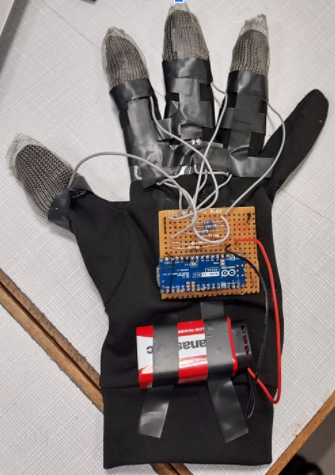
\includegraphics[width=0.3\textwidth]{imgs/Gant.png}
            }

            {\large \ \\ Team: Thibaut Cailleriez, Jean-Edouard Dupau, Pierre Marié, Alondra Alfaro et \bf Florent Pollet\ \\}
            {\large \ \\ Supervisors: \bf Cyril Joly et Bodgan Stanciulescu\ \\}
            \vspace{1cm}
            {\@date\\}

        \end{center}

        \begin{remerciements}
            Je tiens à remercier les encadrants Cyril Joly et Bogdan Stanciulescu pour 
             l'organisation des conférences avec des intervenants de centres de recherche et d'entreprises,
             leurs cours passionnants d'électronique embarquée
             et leur aide ainsi que leur encadrement tout au long du projet.
            Cela a été une expérience très formatrice et intéressante de travailler en équipe à la réalisation d'un prototype
             fonctionnel en un temps restreint.
        \end{remerciements}
    
    
        \tableofcontents

    \end{titlepage}
        

    \newpage

    \makeatother

    
    \tableofcontents

    \section{Introduction}

        Ce projet est issu d'une excellente idée de Thibaut.

        \subsection{Cahier des charges}

        Le concept du projet à formaliser a été de proposer un gant "connecté", 
            c'est-à-dire pouvant contrôler par des gestes les objets connectés du quotidien,
            qui occupent une place croissante dans nos foyers. L'existence d'API majeures comme celles
            de Google Home ou Amazon Alexa laissent supposer une possibilité de contrôle standardisée
            des objets connectés, c'est pourquoi il pourrait être intéressant d'explorer cette
            potentielle opportunité.

        Nous proposerions donc un produit qui répondrait à un besoin naissant de contrôle simple des nouveaux
            éléments de notre environnement. Certes, l'usage actuel reposant sur des applications mobiles
            semble être bien adopté, toutefois un gant restant en permanence sur la main chez soi peut être plus
            simple et plus naturel, ce qui aiderait et favoriserait le développement de la domotique.

        Après échange avec nos encadrants et recherches sur Internet, nous avons défini un Minimum Viable Product (MVP)
            à réaliser pour le projet, l'objectif n'étant pas complémentement d'en faire un objet déjà
            "commercialisable" :
            \begin{itemize}
                \item Les objets à contrôler sont des lampes (on/off) et une enceinte (play/pause) grâce à une API classique.
                \item La zone à couvrir est une pièce de taille moyenne.
                \item Les gestes à détecter sont une main qui pointe ou un doigt en contact avec le pouce.
                \item Il faut être capable de connaitre la localisation et l'orientation du gant pour pouvoir
                        récupérer la position de ce qui est pointé
                        avant de faire un geste qui exécute un ordre.
                \item Il est possible d'utiliser un intermédiaire entre le gant et les objets pour communiquer avec l'API.
            \end{itemize}

        J'ai eu deux rôles au cours du projet, en plus de participer activement à la motivation et à l'organisation grâce à des 
            échanges fréquents sur une conversation Messenger :
            \begin{itemize}
                \item Tout d'abord, nous avons développé des modules séparément après la définition du cahier des charges et des choix techniques.
                        Sur certaines parties difficiles, nous avons choisi de travailler en binôme pour s'aider mutuellement.
                        \begin{itemize}
                            \item Alondra et Pierre ont travaillé sur le capteur de pression et le contact entre les doigts.
                            \item Thibaut a étudié la triangulation pour la localisation du gant et a réalisé de nombreuses soudures
                                    en aidant Alondra et Pierre.
                            \item Jean-Edouard a beaucoup aidé Thibaut et a travaillé sur le bluetooth classique.
                            \item J'ai travaillé sur différents modules.
                        \end{itemize} 
                \item Pendant un peu plus d'une semaine, je me suis ensuite chargé de réaliser le code pour la fusion de modules développés par les autres membres de l'équipe.
                        Thibaut et Jean-Edouard m'ont aidé pour cette tâche qui demande de bien se mettre d'accord sur les conventions.
                        Pendant ce temps, Alondra et Pierre ont travaillé sur la fin de la formalisation du cahier des charges
                            et la préparation des slides.
            \end{itemize}
               
        \subsection{Montages électroniques et morceaux de code}

            Les principaux montages électroniques que j'ai réalisé pour tester les différents modules sont :

            \begin{itemize}
                \item Une Arduino Uno avec un composant Steval MKI109v3 via I2C.
                    Ce capteur contient la même centrale inertielle que l'Arduino Nano BLE que nous allons utiliser.
                \item Une Arduino Uno avec un composant Bluetooth HC05.
                \item Une Raspberry-Pi configurée pour pouvoir utiliser SSH et VNC.
            \end{itemize}

            D'autres montages ont été réalisé par les autres membres de l'équipe :
            \begin{itemize}
                \item Arduino Nano avec capteur de pression (et résistances).
                \item Arduino Nano avec capteur de contact (fils à mettre en contact).
                \item La réalisation d'un support 3D pour les manettes de Wii à placer sur un trépied pour appareil photo.
            \end{itemize}

            Certains montages ont été tentés mais n'ont pas fonctionné :
            % enlever filtre IR Raspberry pi
            \begin{itemize}
                \item Arduino Uno avec la caméra infrarouge (IR) d'une manette de Wii non officielle via I2C et SPI.
                \item Raspberry Pi avec un module caméra sans filtre IR (le filtre n'a pas pu être enlevé).
            \end{itemize}

            En ce qui concerne le code, j'ai créé les dépôts GitHub et je les ai organisés. J'ai codé les modules suivants :
            \begin{itemize}
                \item Communication BLE de l'Arduino Nano BLE (en tant que serveur).
                \item Communication BLE de la Raspberry Pi (en tant que client).
                \item Détermination de l'orientation du gant avec l'Arduino Uno (avec le module Steval) puis avec l'Arduino Nano BLE.
                \item Communication avec Home Assistant sur la Raspberry Pi (via Wifi).
                \item Communication avec MQTT entre différentes Raspberry Pi (via Wifi).
                \item J'ai recodé une partie du module de triangulation avec les formules fournies par Thibaut.
            \end{itemize}

            J'ai également réalisé l'installation et la configuration du serveur Home Assistant sur la Raspberry Pi, ainsi 
            que de MQTT.

    \section{Réalisation du projet}

            Pour réaliser ce gant connecté, nous avons disposé de 5 semaines.

            Ce délai a imposé de prendre des décisions très rapidement concernant les choix techniques
                pour avoir le temps de commander les composants sur différentes plateformes.
            Nous avons fait face à certaines ruptures de stock qui nous ont conduit à commander sur 
                des plateformes différentes (où cela était en stock).
            Une étape compliquée a été la récupération de manettes de Wii officielles après l'échec
                de celles achetées (non officielles).

            L'organisation choisie a été de parallèliser aux maximum les opérations, en commençant par les tests élémentaires
                afin de valider ou infirmer les choix techniques et corriger le plus rapidement la trajectoire du projet,
                en rassemblant au fur et à mesure ce qui fonctionne.

        \subsection{Sélection et obtention des composants}
        
            Nous avons choisi d'utiliser un système une Arduino et une Raspberry
                au lieu d'un seul microcontroleur ou Raspberry afin d'améliorer la portabilité du gant
                (alimentation, poids, puissance de calcul a posteriori).           
            
            % réellement le cas ?

            Afin de simplifier les circuits, j'ai participé au choix de l'Arduino Nano BLE
                qui dispose d'une centrale inertielle et d'un module Bluetooth BLE intégré.

            Les capteurs de pression et de contact ont été sélectionnés.

            Le plus difficile a été le choix de la méthode de triangulation et donc des composants associés.
                Des capteurs Bluetooth prometteurs ont été identifiés mais leur coût (2000 €) a été prohibitif.
                Un système de traitement d'images avec des caméras a été évoqué, mais les données à transférer
                et les algorithmes à utiliser sont complexes.
                Finalement, nous avons choisi d'utiliser les caméras IR des manettes de Wii avec des LED IR 940 nm
            pour trianguler. Les manettes non officielles n'ont cependant pas fonctionné, ce qui nous a fait
            perdre beaucoup de temps entre les essais et la recherche de manettes officielles, malgré de nombreux essais
                de démonter la manette et de récupérer les composants.        

        \subsection{Installation des biliothèques logicielles}

            Pour connecter en Bluetooth (classique) et communiquer avec les manettes Wii (qui donnent directement le point infrarouge sur les coordonnées d'un écran),
                la librairie cwiid a été utilisée. Il a fallu recompiler le wrapper car la version disponible ne fonctionnait pas, la librairie commençant à vieillir
                étant donné l'âge des manettes Wii.           

            Les bibliothèques bluetooth, bleak (pour le BLE), homeassistant (pour la communication avec l'API), MQTT ont dues être installées et être prises en main pour l'intégrer 
                au projet. Le plus gros obstacle était le manque de documentation pour certaines parties.

            L'Arduino a aussi nécessité des bibliothèques pour les capteurs et la BLE.
                Le manque d'information sur les composants a rendu cette tâche parfois difficile et nous ne sommes pas 
                parvenu à trouver des informations sur le capteur des manettes non officielles.
            Nous avons envisagé d'utiliser OpenMV pour programmer l'Arduino en Python mais cela s'est révélé trop compliqué
                et nous avons préféré suivre une voie plus traditionnelle.
            
            % compilation à la main du wrapper cwiid
        \subsection{Création d'objets connectés}

            Afin de tester notre projet, nous avons dans un premier temps créé des objets connectés de type LED/Lampe
                avec une Raspberry Pi (car le Bluetooth et Python sont intégrés), toutefois nous avons dans un second temps
                reproduit le même objet avec uniquement une Arduino Uno et son module Bluetooth.
            
            Finalement, nous avons utilisé de vraies ampoules et enceinte connectées pour nos tests, nous ne nous en sommes donc pas servis.

        \subsection{Communication entre les objets}

            Pour utiliser les lampes connectées, qui sont nativement gérées par l'application Smart Life, il a fallu se créer un compte développeur
                et générer un token à insérer dans Home Assistant. Il peut ainsi communiquer avec Smart Life et agir sur tous les objets qui y sont reliés.

            La solution avec MQTT pour les objets connectés fabriquées n'a pas été conservée mais très intéressante à implémenter.

            Pour l'enceinte Bluetooth, Jean-Edouard s'est chargé de développer le code qui communique avec elle.

        \subsection{Orientation du gant à l'aide de la centrale inertielle}

            Cette partie m'a demandé de lire un peu plus de théorie.

            J'ai comparé plusieurs méthodes qui utilisaient une partie ou l'intégration des neufs degrés de liberté de la centrale inertielle :
            \begin{itemize}
                \item Une première méthode sans calibration : les résultats sont aberrants et non exploitables.
                \item Une méthode sans intégration mais avec un programme pour une calibration extérieure. C'est celle qui a donné de meilleures résultats 
                        qui sont plutôt exploitables pour une très faible précision.
                \item Une méthode avec intégration (par exemple Madgwick) : il m'a manqué du temps pour régler tous les paramètres avec d'obtenir des résultats satisfaisants.
            \end{itemize}
            
            Le passage de l'Arduino Uno avec Sterval à la Nano a demandé une adaptation imprévue et conséquente du code car la bibliothèque n'était pas exactement similaire
                (dernières mises à jour non présentes).
            
            
        \subsection{Réalisation du gant}
            Cette partie a été réalisée en parallèle par d'autres membres de l'équipe. 
            Je n'ai que été chargé de mettre le code ensemble et de le téléverser sur l'Arduino Nano, cela a cependant demandé
                de nombreux ajustements afin que tout fonctionne, en plus du recodage d'une partie de l'algorithme de triangulation.
            J'ai ainsi peu souder, à part pour aider Thibaut à quelques occasions.

    \section{Conclusion}

            Le MVP iGlove a ainsi pu être atteint comme l'a montré la démonstration et cela pourrait servir de Proof of Concept (POC) pour un nouveau produit
             toutefois il reste de nombreux ajustements à réaliser sur les aspects étudiés pour élargir le champ des possibles et les fonctionnalités du gant :
             \begin{itemize}
                \item La triangulation est encore trop imprécise, il faudrait estimer l'incertitude miminum théorique atteignable 
                        pour savoir si nous pouvons encore continuer de s'appuyer sur cette méthode.
                \item Le magnétomètre est fortement perturbé en intérieur malgré une calibration extérieure.
                        Il faudrait mieux gérer les appareils électromagnétiques en intérieur.
                \item Le calibrage est encore trop long et fastidieux pour un utilisateur néophyte (mesure de distance, placement précis...) :
                        davantage d'automatisation serait nécessaire.
                \item Dans le même domaine, l'uniformisation des protocoles dans les objets connectés est encore imparfaite.
             \end{itemize}

             % quoi en plus ?

    \appendix

    \section {Code source}
        Les codes de l'Arduino et de la Raspberry Pi sont disponibles aux adresses suivantes :
        \begin{itemize}
            \item \url{https://github.com/florian6973/iglove-arduino}
            \item \url{https://github.com/florian6973/iglove-pi}
        \end{itemize}
\end{document}
